\documentclass[french, 9pt]{article}

%-------------------------------------------------------------------------------
\usepackage[a4paper,top=1cm,bottom=2cm,left=1cm,right=1cm,marginparwidth=0.5cm]{geometry}
\usepackage{amsmath,amsfonts,amssymb,amsthm}
\usepackage[french]{babel}
\usepackage[utf8]{inputenc}
\usepackage[T1]{fontenc}
\usepackage{enumerate}
\usepackage{natbib}
\usepackage{graphicx}
\usepackage{xspace}
\usepackage{color,xcolor}
\usepackage{tikz}
\usepackage{remreset}
\usepackage{url}
\usepackage{boites}
% \usepackage{extsizes} % Permet \documentclass[french, 14pt]{extreport}
% \usepackage[a4paper,top=1cm,bottom=2cm,left=1cm,right=1cm,marginparwidth=.75cm]{geometry}
% \usepackage{minitoc}

\graphicspath{{../Figures/}}
% Environnement
\newtheorem{theorem}{Théorème}
\newtheorem{definition}{Définition}
\newtheorem{lemma}{Lemme}
\newtheorem{proposition}{Proposition}
\newtheorem*{theorem*}{Théorème}
\newtheorem*{definition*}{Définition}
\newtheorem*{proposition*}{Proposition}
\newtheorem*{corollary*}{Corollaire}
\newtheorem*{assumption*}{Hypothèse}
\newtheorem*{algorithm*}{Algorithme}
\newtheorem*{lemma*}{Lemme}
\newtheorem*{remark*}{Remarque}
\newtheorem*{exercise*}{Exercice}
\newtheorem{exercise}{Exercice}
\newcommand{\remark}{\bigskip\noindent\textbf{\textsl{Remarque.}}\xspace}
\newcommand{\remarks}{\bigskip\noindent\textbf{\textsl{Remarques.}}\xspace}
\newcommand{\parSR}[1]{\paragraph*{\textsl{#1}}\xspace}
\renewcommand{\proof}{\bigskip\noindent\underline{\textsl{Démonstration}.}\xspace}
\newcommand{\eproof}{$\blacksquare$}

% Effets, couleurs
\newcommand{\emphase}[1]{\textcolor{red}{#1}}
\newcommand{\demoProp}[1]{\noindent{\textbf{\textsl{Démonstration de la proposition \ref{#1} :}}}}
\newcommand{\itemdot}{\textbullet}

% Moments
\DeclareMathOperator{\Esp}{\mathbb{E}}
\DeclareMathOperator{\diag}{diag}
\DeclareMathOperator{\Cov}{\mathbb{C}ov}
\DeclareMathOperator{\tr}{tr}
\DeclareMathOperator{\Var}{\mathbb{V}}
\let\Pr\relax\DeclareMathOperator{\Pr}{\mathbb{P}}
\renewcommand{\d}{\text{d}}

% R, N, ...
\newcommand{\cst}{\text{cst}}
\newcommand{\Cbb}{\mathbb{C}}
\newcommand{\Ibb}{\mathbb{I}}
\newcommand{\Nbb}{\mathbb{N}}
\newcommand{\Rbb}{\mathbb{R}}
\newcommand{\Zbb}{\mathbb{Z}}

% Indicateurs

% Lois et ensembles
\newcommand{\Acal}{\mathcal{A}}
\newcommand{\Bcal}{\mathcal{B}}
\newcommand{\Ccal}{\mathcal{C}}
\newcommand{\Ecal}{\mathcal{E}}
\newcommand{\Gcal}{\mathcal{G}}
\newcommand{\Ical}{\mathcal{I}}
\newcommand{\Lcal}{\mathcal{L}}
\newcommand{\Mcal}{\mathcal{M}}
\newcommand{\Ncal}{\mathcal{N}}
\newcommand{\Pcal}{\mathcal{P}}
\newcommand{\Rcal}{\mathcal{R}}
\newcommand{\Scal}{\mathcal{S}}
\newcommand{\Ucal}{\mathcal{U}}
\newcommand{\Xcal}{\mathcal{X}}
\newcommand{\Ycal}{\mathcal{Y}}

% Comments
\newcommand{\SR}[2]{\textcolor{gray}{#1}\textcolor{red}{#2}}
\newcommand{\todo}[1]{\textcolor{red}{\`A faire~: {\sl #1}}}
\newcommand{\dessin}[1]{
\begin{center}\framebox{\begin{minipage}{\textwidth}
  \textcolor{purple}{#1}
\end{minipage}}\end{center}
\bigskip
}
\newcommand{\progres}[1]{
\begin{center}\framebox{\begin{minipage}{\textwidth}
  \textcolor{blue}{{\sl #1}}
\end{minipage}}\end{center}
\bigskip
}
\newcommand{\solution}[1]{
\begin{center}\framebox{\begin{minipage}{\textwidth}
  \noindent{\sl Solution :}
  #1
\end{minipage}}\end{center}
\bigskip
}
% \newcommand{\exemple}[1]{
% \begin{center}\framebox{\begin{minipage}{\textwidth}
%   \parSR{Exemple.}
%   #1
% \end{minipage}}\end{center}
% \bigskip
% }
\newcommand{\exemple}[1]{
\begin{breakbox}
  \parSR{Exemple.}
  #1
\end{breakbox}
\bigskip
}

\newcommand{\SRcorrect}[2]{\textcolor{gray}{#1}\textcolor{blue}{#2}}
\newcommand{\SRcomment}[1]{\textcolor{blue}{[{\sl SR: #1}]}}



% Section numbering
\usepackage{chngcntr}
\renewcommand{\thepart}{\Roman{part}}
% \counterwithout{section}{part}
\setcounter{secnumdepth}{3}
\setcounter{tocdepth}{1}

% Proposition numbering
\renewcommand{\subsubsection}{\section}
% \numberwithin{exercise}{section}
% \numberwithin{equation}{section}

% Suppression des solutions
% \renewcommand{\solution}[1]{}

\newcommand{\alglin}{/home/robin/ENSEIGN/Cours/MathBiologie/L3-ENS-Math1/Exercices/AlgLin}
\newcommand{\multivar}{/home/robin/ENSEIGN/Cours/MathBiologie/L3-ENS-Math1/Exercices/MultiVar}
\newcommand{\equadiff}{/home/robin/ENSEIGN/Cours/MathBiologie/L3-ENS-Math1/Exercices/EquaDiff}
\newcommand{\probas}{/home/robin/ENSEIGN/Cours/MathBiologie/L3-ENS-Math1/Exercices/Probas}


% %-------------------------------------------------------------------------------
% %-------------------------------------------------------------------------------
% \title{\Huge{Ce qu'un biologiste doit savoir en mathématiques}}
% \author{SR d'après \cite{Lam20} : Annexes}
% \date{\today}


\title{\normalsize{\sc École Normale Supérieure de Paris, Licence de Biologie L3}
  
  \bigskip
  \normalsize{\sc Année 2023–24}
  
  \bigskip
  \large{\bf Mathématiques I : ce qu’un biologiste ne doit pas ignorer} 
  
}
\date{Examen oral, le 12 février 2024}

%-------------------------------------------------------------------------------
%-------------------------------------------------------------------------------
\begin{document}
%-------------------------------------------------------------------------------
%-------------------------------------------------------------------------------

\maketitle

\bigskip
Les notes de cours individuelles sont autorisées.
L’usage de tout appareil électronique est interdit à l’exception d’une calculatrice.

%-------------------------------------------------------------------------------
% \section{Algèbre linéaire}
% %-------------------------------------------------------------------------------
\subsubsection{Dynamique d'une population de Leslie}
%-------------------------------------------------------------------------------

% Cf exercice 5 AL

On considère une population structurée en $n$ classes d'âge. Pour $1 \leq i \leq n$, on note $x_k(t)$ le nombre d'individus de la classe $k$ à la génération $t$ et $x(t) = [x_1(t) \dots x_n(t)]^\top$ le vecteur décrivant l'ensemble de la population à cette même génération. On suppose que l'évolution de cette population est régit par la récurrence
\begin{equation} \label{eq:recurrenceLeslie}
  x(t+1) = A x(t)
\end{equation}
où $A$ est la matrice de Leslie
$$
A = \left[\begin{array}{cccccc}
            f_1 & f_2 & \cdots  & \cdots & f_n \\
            s_1 & 0 & \cdots  & \cdots & 0 \\
            0 & \ddots  & \ddots & & \vdots \\
            \vdots & \ddots & \ddots & \ddots & \vdots \\
            0 & \cdots & 0 & s_{n-1} & 0 \\
          \end{array}\right]
$$
où tous les coefficients $f_i$ et $s_i$ sont supposés strictement positifs. On note de plus
$$
\ell_1 = 1 \qquad \text{et} \qquad 
\ell_k = \prod_{i=1}^{k-1} s_i \quad \text{pour $2 \leq k \leq n$}.
$$

\begin{enumerate}
  \item Interprêter les coefficients $f_i$ et $s_i$.
  \solution{$f_i$ est le taux de fertilité de la classe $i$ (qui alimente la classe 1). $S_i$ est le taux de survie de la classe $i$ (qui alimente la classe $i+1$).}
  %
  \item Soient $B_{k1} \in \Mcal_{k-1}$, $B_{k2} \in \Mcal_{n-k}$ définies par :
  $$
  B_{k1} = \left[\begin{array}{cccc}
            s_1 & -\lambda & &  \\
            & \ddots & \ddots & \\
            & & \ddots & -\lambda \\
            & & & s_{k-1}
          \end{array}\right], \qquad
  B_{k2} = \left[\begin{array}{cccc}
            -\lambda & & & \\
            s_{k+1} & \ddots & & \\
            & \ddots & \ddots & \\
            & & s_{n-1} & -\lambda
          \end{array}\right].
  $$
  En notant $0_{p,q}$ la matrice $p \times q$ dont tous les éléments sont nuls, calculer le déterminant de la matrice $B_k \in \Mcal_{n-1}$ :
  $$
  B_k = \left[\begin{array}{cc}
            B_{k1} & 0_{k-1, n-k} \\
            0_{n-k, k-1} & B_{k2}
          \end{array}\right].
  $$
  \solution{On utilise le calcul du déterminant par bloc pour obtenir
  $$
  |B| = |B_{k1}| \times |B_{k2}|
  $$
  et on remarque que, puisque $B_{k1}$ et $B_{k2}$ sont respectivement triangulaires supérieure et inférieure, leurs déterminants sont égaux au produit de leurs termes diagonaux, soit
  $$
  |B_{k1}| = \ell_k, \qquad |B_{k2}| = (-\lambda)^{n-k}.
  $$
  }
  %
  \item Montrer que le polynôme caractéristique de $A$ est
  $$
  P_A(\lambda) = (f_1 - \lambda) (-\lambda)^{n-1} + \sum_{k=2}^{n} (-1)^{k-1} f_k \ell_k (-\lambda)^{n-k}.
  $$
  \solution{Les termes successifs du développement du déterminant 
  $$
  |A - \lambda I| 
  = \left|\begin{array}{cccccc}
            f_1-\lambda & f_2 & \cdots  & \cdots & f_n \\
            s_1 & -\lambda & 0  & \cdots & 0 \\
            0 & s_2 & \ddots & \ddots & \vdots \\
            \vdots & \vdots & \ddots & \ddots & 0 \\
            0 & \cdots & 0 & s_{n-1} & -\lambda \\
          \end{array}\right|
  $$ 
  par rapport à la première ligne sont
  \begin{align*}
  (f_1 - \lambda) |B_1| & = (f_1-\lambda) (-\lambda^{n-1}), &
  - f_2 |B_2| & = -f_2 s_1 (-\lambda)^{n-2}, \\
  f_3 |B_3| & = f_3 s_1 s_2 (-\lambda)^{n-3}, & 
  -f_4 |B_4| & = -f_4 s_1 s_2 s_3 (-\lambda)^{n-4}, \qquad \dots
  \end{align*}
  }
  %
  \item En déduire que la plus grande valeur propre en module $\lambda_1$ de la matrice $A$ vérifie
  $$
  \sum_{k=1}^n \ell_k f_k \lambda_1^{-k} = 1.
  $$
  \solution{Toutes les valeurs propres, dont $\lambda_1$, sont solutions de $P_A(\lambda) = 0$, soit
  \begin{align*}
  (f_1 - \lambda) (-\lambda)^{n-1} + \sum_{k=2}^{n} (-1)^{k-1} f_k \ell_k (-\lambda)^{n-k} & = 0 \\
  \Leftrightarrow \qquad \sum_{k=1}^n (-1)^{k-1} f_k \ell_k (-\lambda)^{n-k} & = (-\lambda)^{n-1} & 
  \Leftrightarrow \qquad \sum_{k=1}^n f_k \ell_k \lambda^k & = 1.
  \end{align*}
  }
\end{enumerate}

On s'intéresse maintenant aux vecteurs propres à gauche et à droite de la matrice $A$. On note 
$$
a = \sum_{k=1}^n \ell_k \lambda_1^{-k}, \qquad
b = \sum_{k=1}^n k \ell_k f_k \lambda_1^{-k}.
$$
\begin{enumerate}
  \setcounter{enumi}{4}
  \item Montrer que le vecteur $v$ de coordonnées
  $$
  v_k = \frac1a \ell_k \lambda_1^{-k}, \qquad 1 \leq k \leq n,
  $$
  est un vecteur propre à droite de $A$ associé à la valeur propre $\lambda_1$.
  \solution{Soit le vecteur $w = Av$. Ses coordonnées sont
  \begin{align*}
    w_1 & = \sum_{k=1}^n f_k v_k = \frac1a \sum_{k=1}^n f_k \ell_k \lambda_1^{-k} = \frac1a = \lambda_1 v_1, \\
    w_k & = s_{k-1} v_{k-1} = \frac1a s_{k-1} \ell_{k-1} \lambda_1^{-k+1}  = \frac1a \ell_k \lambda_1^{-k+1} = \lambda_1 v_k, \qquad \text{pour $2 \leq k \leq n$}.
  \end{align*}
  }
  \item Montrer que le vecteur $u$ de coordonnées
  $$
  u_k = \frac1{b v_k} \sum_{j=k}^n \ell_j f_j \lambda_1^{-j}, \qquad 1 \leq k \leq n,
  $$
  est un vecteur propre à gauche de $A$ associé à la valeur propre $\lambda_1$.
  \solution{Soit le vecteur $w^\top = u^\top A$. On a
  $$
  w_n = f_n u_1
    = f_n \frac{a \lambda_1}b \sum_{j=1}^n \ell_j f_j \lambda_1^{-j}
    = f_n \frac{a \lambda_1}b
  $$
  or
  $$
  u_n = \frac{\ell_n f_n \lambda_1^{-n}}{b v_n} = \frac{a f_n}{b}, 
  \qquad \text{donc} \quad w_n = \lambda_1 u_n.
  $$
  De plus, pour $1 \leq k \leq n-1$, on a
  \begin{align*}
    w_k & = f_k u_1 + s_k u_{k+1} 
    = f_k \frac{a \lambda_1}{b} \sum_{j=1}^n \ell_j f_j \lambda_1^{-j} + s_k \frac{a \lambda_1^{k+1}}{b \ell_{k+1}} \sum_{j=k+1}^n \ell_j f_j \lambda_1^{-j} \\
    & = \frac{a \lambda_1^{k+1}}{b \ell_k} \left(f_k \ell_k \lambda_1^{-k} + \sum_{j=k+1}^n \ell_j f_j \lambda_1^{-j}\right)
    = \lambda_1 \frac{a \lambda_1^k}{b \ell_k} \sum_{j=k}^n \ell_j f_j \lambda_1^{-j}
    = \lambda_1 u_k.
  \end{align*}}
\end{enumerate}

On s'intéresse enfin au comportement asymptotique du vecteur $x(t)$ décrivant la composition de la population au bout de $t$ générations.
\begin{enumerate}
  \setcounter{enumi}{6}
  \item Calculer $\sum_{k=1}^n v_k$ et $\sum_{k=1}^n v_k u_k$.
  \solution{On a
  \begin{align*}
    \sum_{k=1}^n v_k 
      & = \frac1a \sum_{k=1}^n \ell_k \lambda_i^{-k} = 1 \\
    \sum_{k=1}^n v_k u_k 
      & = \frac1b \sum_{k=1}^n \sum_{j=k}^n \ell_j f_j \lambda_1^{-j}
      = \frac1b \sum_{k=1}^n k \ell_k f_k \lambda_1^{-k} = 1.
  \end{align*}}
  \item Partant d'un vecteur de composition initial $x(0)$, quel est le comportement asymptotique de $x(t)$ quand $t$ tend vers l'infini ?
  \solution{La récurrence \eqref{eq:recurrenceLeslie} implique que $x(t) = A^t x(0)$. De plus, le théorème de Perron-Frobénius nous assure que $\lim_{t \to \infty} \lambda_1^{-t} A^t = v u^\top$. On a donc
  $$
  \lim_{t \to \infty} \lambda_1^{-t} x(t) 
  = \lim_{t \to \infty} \lambda_1^{-t} A^t x_0(t)
  = v u^\top x(0) = \left(u^\top x(0)\right) v
  $$
  soit $x(t) \approx c_0 \lambda_1^t v$, avec $c_0 = u^\top x(0)$.
  \begin{itemize}
   \item La taille totale de la population évolue asymptotiquement comme $\lambda_1^n$. 
   \item La composition asymptotique relative de la population est donnée par les coordonnées du vecteur $v$ (qui somment à 1). 
   \item Le produit scalaire $c_0$ indique comment les effectifs initiaux $x_k(0)$ contribuent respectivement (à proportion de $u_k$) à la taille asymptotique de la population.
  \end{itemize}}
\end{enumerate}


%-------------------------------------------------------------------------------
% \section{Fonction de plusieurs variables}
% %-------------------------------------------------------------------------------
\subsubsection{Exemple de fonction de $\Rbb^2 \mapsto \Rbb$}
%-------------------------------------------------------------------------------

Soit la fonction $f: \Rbb^2 \mapsto \Rbb$ définie par
$$
f(x, y) = x^3 + y^3 - 3 xy
$$

\begin{enumerate}
  \item Déterminer les points stationnaires de la fonction $f$.
  \solution{
    Le gradient de $f$ vaut
    $$
    \nabla f = \left[\begin{array}{c} 3x^2 - 3y \\ 3y^2 - 3x \end{array}\right]
    $$
    qui est nul aux points
    $$
    a = (0, 0) \qquad \text{et} \qquad b = (1, 1).
    $$
  }
  \item Déterminer s'il s'agit de maximums, de minimums ou de points selles.
  \solution{
    La hessienne vaut
    $$
    \nabla^2 f = \left[\begin{array}{rrr} 6x & & -3 \\ -3 & & 6y \end{array}\right].
    $$
    \begin{description}
      \item[\'Etude du point $a$ :] on a 
      $$
      \nabla_a^2 f = \left[\begin{array}{rrr} 0 & & -3 \\ -3 & & 0 \end{array}\right]
      \qquad \Rightarrow \qquad 
      | \nabla_a^2 f | = -9 < 0
      $$
      donc $a$ est un point selle. Ses valeurs propres sont les racines de
      $$
      P(\lambda) = \left|\begin{array}{rrr} -\lambda & & -3 \\ -3 & & -\lambda \end{array}\right|
      = \lambda^2 - 9 
      \qquad \text{soit} \quad 
      \lambda = \pm 3.
      $$
      Tout vecteur propre associé à $\lambda = -3$ est solution de 
      $$
      \left\{\begin{array}{rcl} -3y & = & -3x \\-3x & = & -3y\end{array} \right.
      \qquad \Rightarrow \qquad 
      x = y
      \qquad \Rightarrow \qquad 
      \left[ \begin{array}{r} 1 \\ 1 \end{array} \right] \text{ est associé à $-3$}
      $$
      donc $a$ est un maximum dans la direction de la 1ère bissectrice. \\
      Tout vecteur propre associé à $\lambda = 3$ est solution de 
      $$
      \left\{\begin{array}{rcl} -3y & = & 3x \\-3x & = & 3y\end{array} \right.
      \qquad \Rightarrow \qquad 
      x = -y
      \qquad \Rightarrow \qquad 
      \left[ \begin{array}{r} -1 \\ 1 \end{array} \right] \text{ est associé à $+3$}
      $$
      donc $a$ est un minimum dans la direction de la 2ème bissectrice.
      $$
      \begin{tabular}{cc}
        direction $x = y$ & direction $x = -y$ \\
        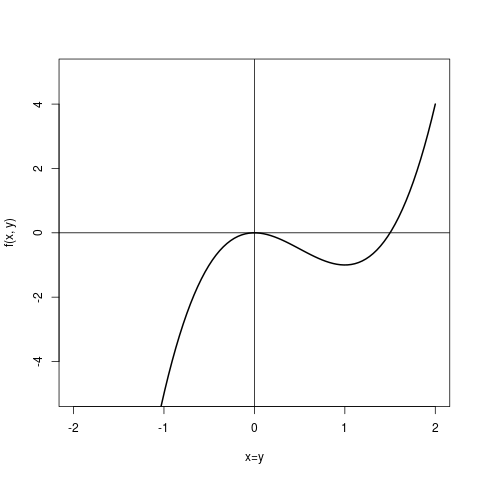
\includegraphics[width=.35\textwidth, trim=00 10 10 40, clip=]{ExempleOptimum-1ereBissectrice} &
        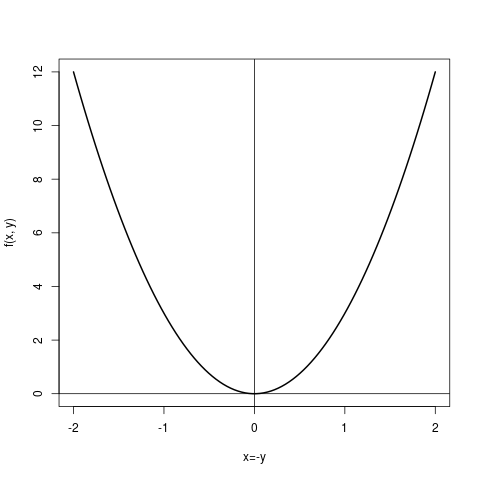
\includegraphics[width=.35\textwidth, trim=00 10 10 40, clip=]{ExempleOptimum-2emeBissectrice} \\
        $f(x, x) = 2x^3 - 3x^2$ & $f(x, -x) = 3x^2$
      \end{tabular}
      $$
      \item[\'Etude du point $b$ :] on a
      $$
      \nabla_b^2 f = \left[\begin{array}{rrr} 6 & & -3 \\ -3 & & 6 \end{array}\right]
      \qquad \Rightarrow \qquad 
      | \nabla_b^2 f | = 27 > 0, \qquad \tr(\nabla_b^2 f) = 12 > 0
      $$
      donc les deux valeurs propres de $\nabla_b^2 f$ sont positives : $b$ est donc un minimum.
    \end{description}
    Au total la surface d'équation $\{z = f(x, y)\}$ a l'aspect suivant
    $$
    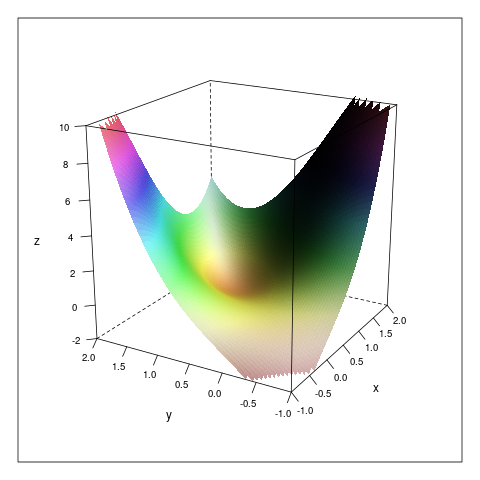
\includegraphics[width=.6\textwidth]{ExempleOptimum-surface}
    $$
  }
\end{enumerate}


%-------------------------------------------------------------------------------
% \section{Systèmes dynamiques}
% \bigskip \bigskip 
\newpage
%-------------------------------------------------------------------------------
\subsubsection{Modèle cubique}
%-------------------------------------------------------------------------------

% [Exercice 2, TD2, L2 Bio SU]

\exemple{
  On considère le système
  $$
  \dot y = - y^3 + 7 y^2 - 14 y + 8.
  $$
  Ses points stationnaires sont les racines du polynôme $P(y) = - y^3 + 7 y^2 - 14 y + 8$, donc $y_1 = 1$ fait partie, donc
  $$
  P(y) = (y-1) (-y^2 + 6y + 8),
  $$
  et les deux racines de $-y^2 + 6y + 8$ sont $2$ et $4$. Les points stationnaires du système sont donc 
  $$
  y_1 = 1, \qquad y_2 = 2, \qquad y_3 = 4.
  $$
  Leur stabilité est donné par la dérivée de $P$:
  $$
  P'(y) = -3y^2 + 14 y - 14,
  $$
  soit
  $$
  P'(y_1) = -3, \qquad P'(y_2) = 2, \qquad P'(y_3) = -6.
  $$
  $y_1$ et $y_3$ sont donc des équilibres stables, et $y_2$ un équilibre instable.
  $$
  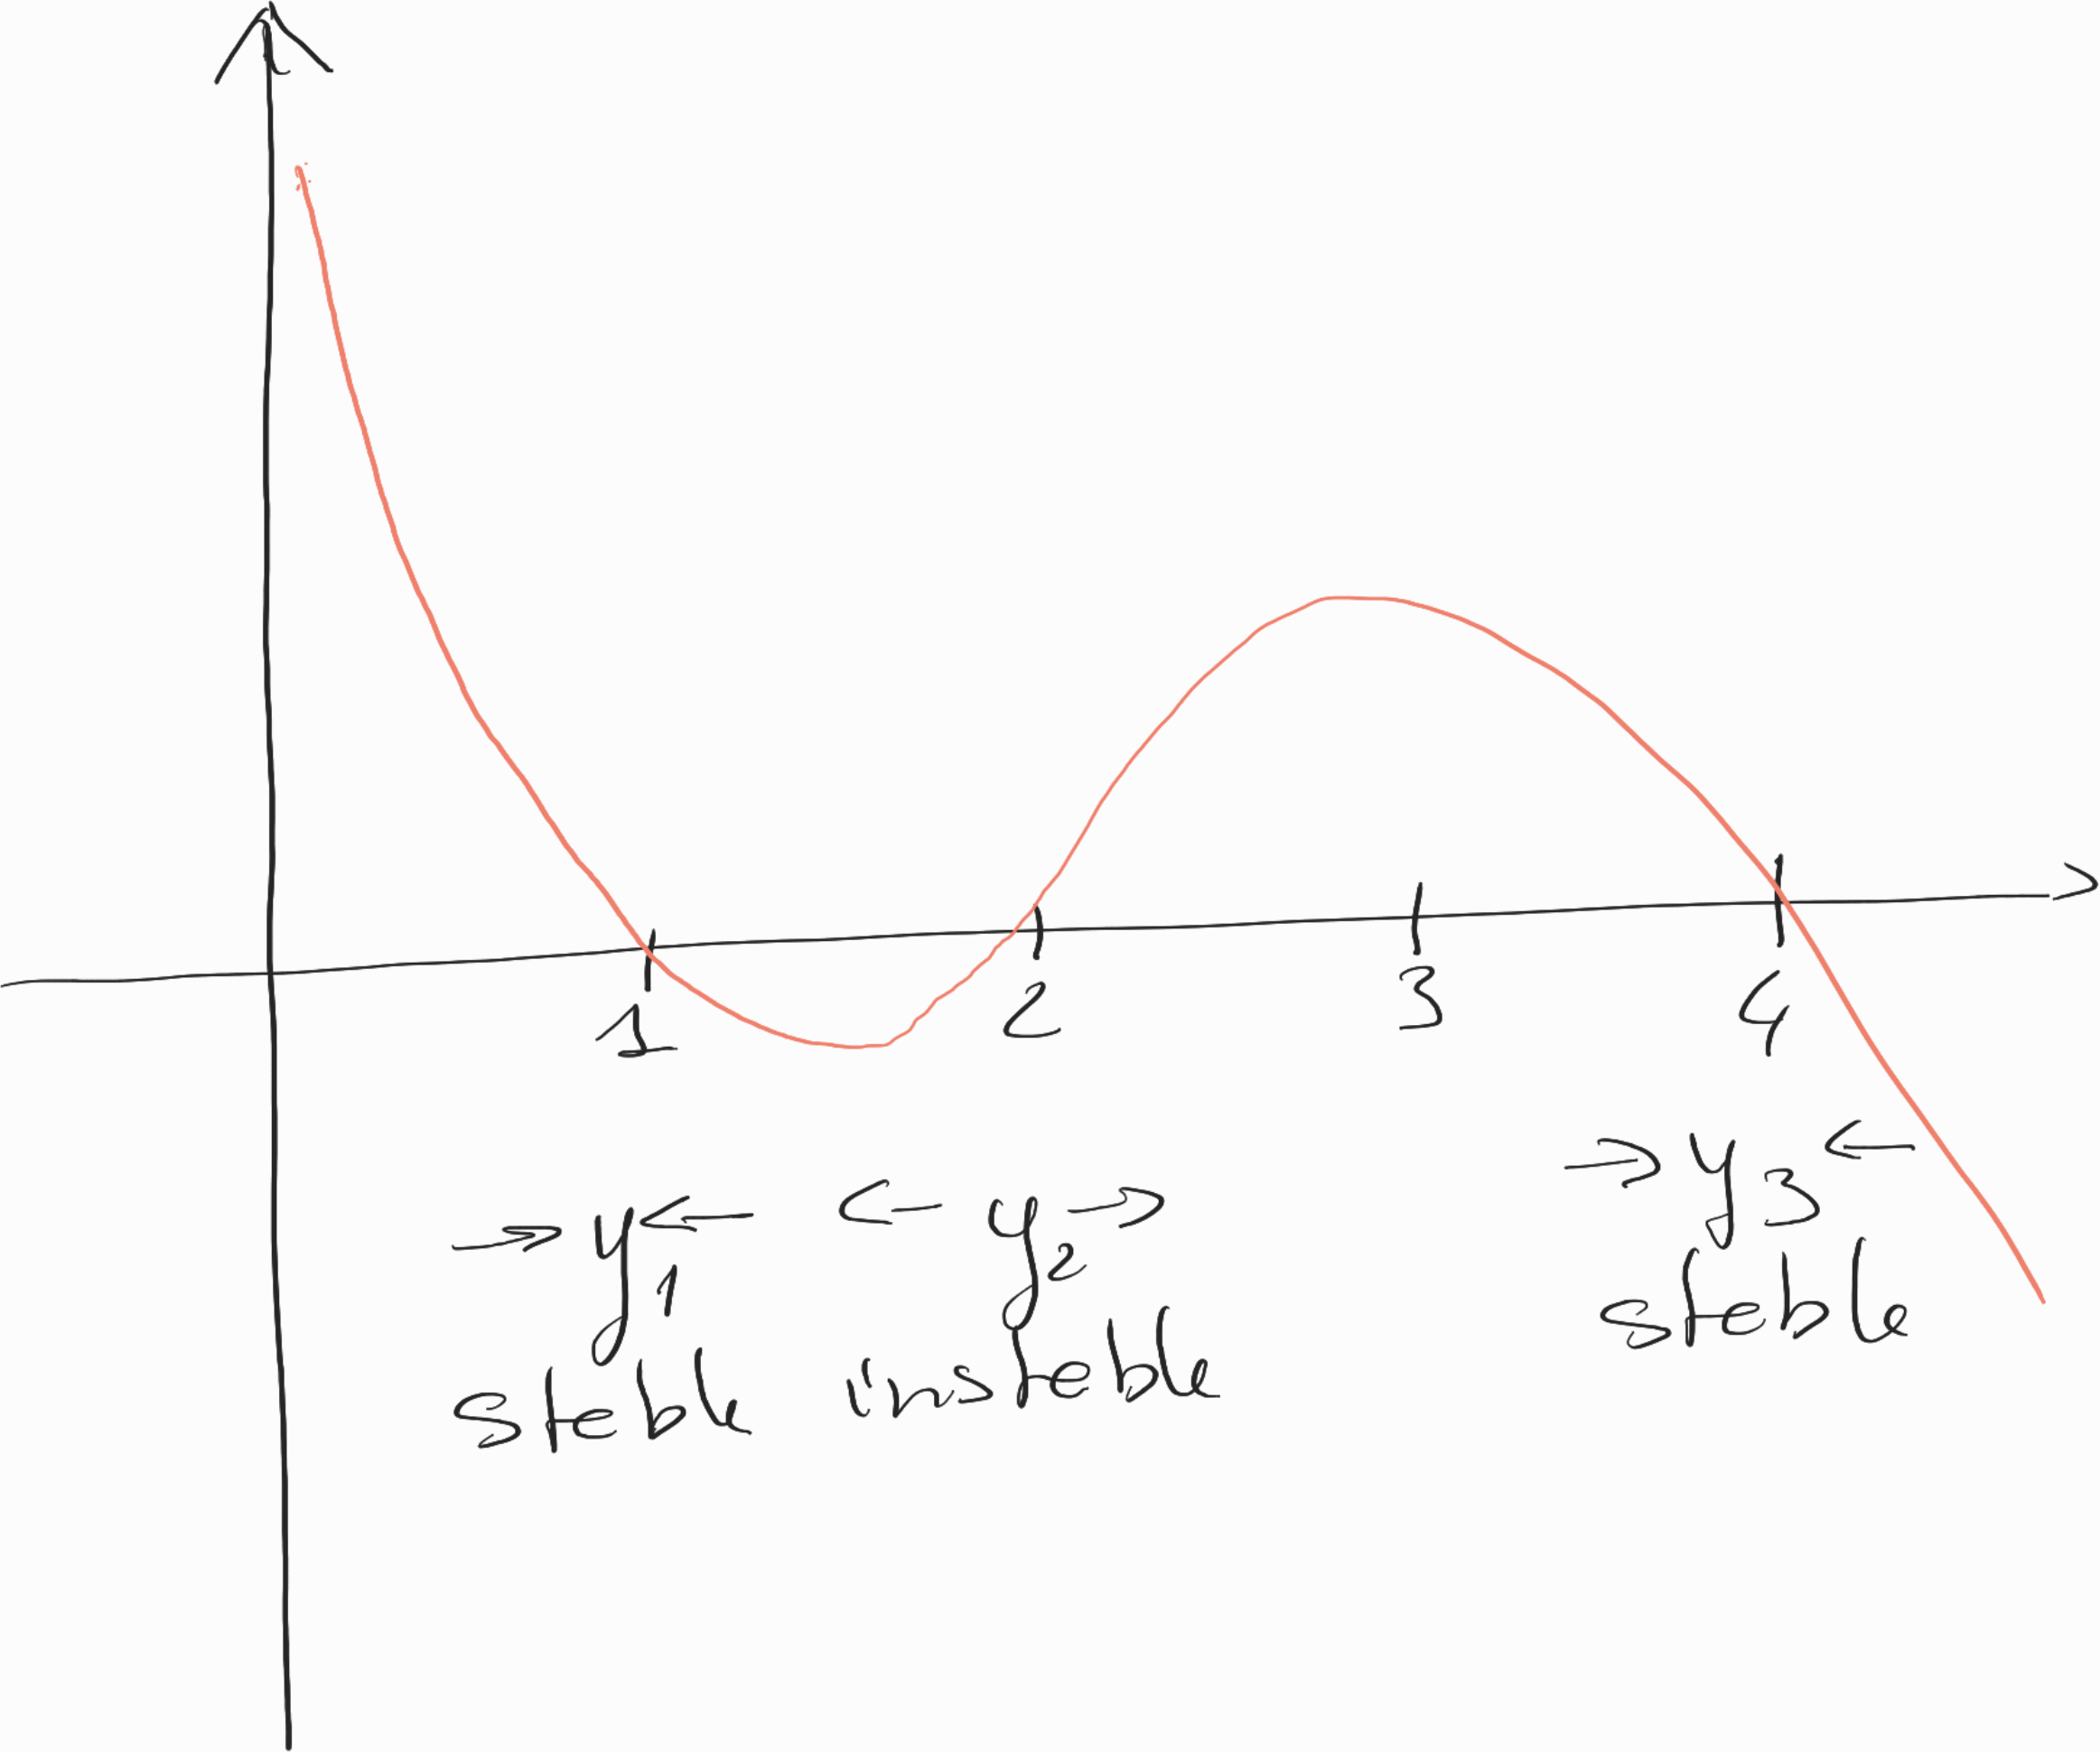
\includegraphics[width=.5\textwidth]{TD-SUbioL3-TD2Exo2}
  $$
}




%-------------------------------------------------------------------------------
% \section{Probabilités}
% \bigskip \bigskip 
\newpage
%-------------------------------------------------------------------------------
\subsubsection{Processus Galton–Watson géométrique avec excès de zéro}
%-------------------------------------------------------------------------------

Les organismes d’une espèce asexuée se reproduisent suivant un processus de Galton–Watson, où chaque individu laisse à la génération suivante un nombre aléatoire $X$ d’individus. \\
On note $p_k = \Pr\{X = k\}$ et on suppose que 
$$
p_0 = b
\qquad \text{et} \qquad 
p_k = (1 - b) (1 - a) a^{k-1} \text{ pour } k \geq 1.
$$
\begin{enumerate}
  \item Montrer que la fonction génératrice de $X$ vaut
  $$
  f(s) := \Esp(s^X) = b + (1-b)(1-a) \frac{s}{1 - as}.
  $$
  \solution{Par définition, on a
  \begin{align*}
    f(s) 
    & =\Esp(s^X) = \sum_{k \geq 0} p_k s^k 
    = b + (1-b) \sum_{\textcolor{red}{k \geq 1}} (1 - a) a^{k-1} s^k \\
    & = b + (1 - b) s \sum_{k \geq 1} (1 - a) (as)^{k-1}
    = b + (1 - b) s \sum_{k \geq 0} (1 - a) (as)^k
  \end{align*}
  où on reconnaît la fonction génératrice d'une variable aléatoire géométrique : 
  $$
  \sum_{k \geq 0} (1 - a) (as)^k = \frac{1 - a}{1 - as},
  $$
  qui donne le résultat.
  }
  \item Déterminer la valeur de la probabilité, notée $q$, qu'une population de cette espèce issue d’un seul individu fondateur s'éteigne.
  \solution{On sait que $q$ est le plus petit point fixe de la fonction $f$ dans l'intervalle $(0, 1]$. Il faut donc résoudre $f(s) = s$
  \begin{align*}
    \Leftrightarrow \qquad 
    b(1 - as) + (1-b)(1-a) s & = a - as^2 \\
    \Leftrightarrow \qquad
    as^2 - (a+b) s + b & = 0
  \end{align*}
  dont le discriminant vaut $\Delta = (a+b)^2 - 4ab = (a-b)^2$ et les solutions sont donc
  $$
  s = \frac{(a+b) \pm (a-b)}{2}
  \qquad \Leftrightarrow \qquad
  s \in \left\{\frac{b}a, 1\right\}.
  $$
  La probabilité d'extinction est donc $q = b/a$ si $b < a$ et 1 sinon.
  }
  \item Par quel autre moyen peut-on déterminer à quelle condition la probabilité d'extinction est strictement inférieure à 1 ?
  \solution{
  On sait que la probabilité d'extinction est strictement inférieure à 1 si le nombre de descendant moyen $m$ est strictement supérieur à 1. Il suffit donc de calculer $m$ pour la loi $p$. \\
  On rappelle l'espérance d'une loi géométrique : si $Z \sim \Gcal(1-a)$, alors
  $$
  \Esp Z 
  = (1-a) \sum_{z \geq 1} z a^{z-1}
  = (1-a) \; \partial_a \left(\sum_{z \geq 0} a^z\right)
  = (1-a) \; \partial_a \left(\frac1{1-a}\right)
  % = (1-a) \frac1{(1-a)^2}
  = \frac1{1-a}.
  $$
  On a donc $m = \Esp X = b \times 0 + (1-b) \Esp Z = (1-b) / (1-a)$ et on retrouve $m > 1 \; \Leftrightarrow \; b < a$.
  }
\end{enumerate}



%-------------------------------------------------------------------------------
%-------------------------------------------------------------------------------
\end{document}
%-------------------------------------------------------------------------------
%-------------------------------------------------------------------------------


